% Book pp. 134-138 (PDF pp. 135-139)
\section*{Geometric Reasoning and Measurement}
\subsection*{Spatial Sense}

\section{Introduction}

In this section, you will learn how to derive the circle equation. You will also
learn how to manipulate this equation under given conditions and apply it to
solve real-life problems. The content of this section is imperative as it forms the
foundation on which other advanced topics in mathematics are built. Its real-life
applications are vast so why not delve further through your own research.

\begin{keyideas}
\begin{itemize}
  \item A circle is a path traced by all points in a plane which are equidistant
  from a fixed point in the plane. The fixed point is called the centre.
  \item The standard equation of a circle with centre $(h, k)$ and radius $r$ is given
  as:
  \item $(x - h)^2 + (y - k)^2 = r^2$
  \item The general equation of a circle with centre $(-g, -f)$ and radius $r$ is
  given as:
  \item $x^2 + y^2 + 2gx + 2fy + c = 0$
\end{itemize}
\end{keyideas}

\section{Exploring the Properties of a Circle and its Parts}

\subsection{A Circle}

The circle is the path traced by all points in a plane which are equidistant from a
fixed point in the plane. The fixed point is called the centre.

Let us use the activity below to revise the parts of the circle. You will need a
graph sheet and a set of mathematical instruments to do this activity.

\begin{activity}{Activity 4.1- Parts of a circle}
\textbf{Step 1:} Make a copy of the graph below.
\begin{center}
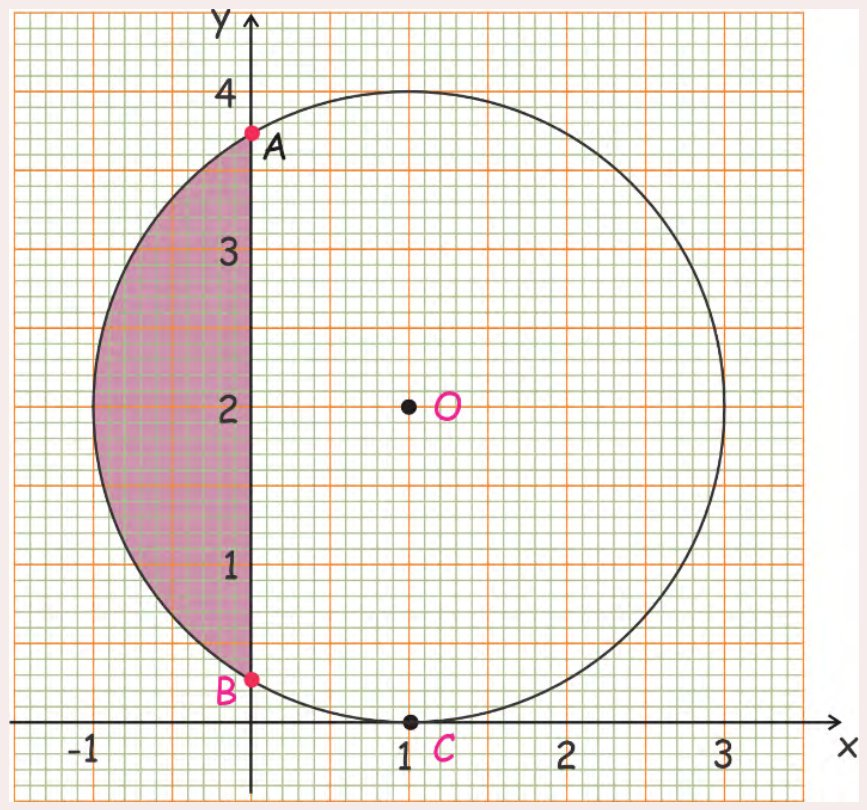
\includegraphics[width=0.6\linewidth]{figures/fig4-1.jpg}
\end{center}
\figcaption{4.1}{A circle}

\textbf{Step 2:} Calculate $|$OA$|$, $|$OB$|$ and $|$OC$|$

\textbf{Step 3:} Comment on any observation from your result in Step 2

\textbf{Step 4:} Aside from points A, B and C, list the coordinates of any two points
on the circle's circumference. Find the distance between these points and
point O. Comment on your observations.

\textbf{Step 5:} Join points O and C with a straight line.

Measure the angle between OC and the $x$-axis.
\end{activity}

\textbf{Let us use our diagram to revise the parts of the circle.}

Lines OA, OB and OC are the radii of the circle. From the activity, $|$OA$|=|$OB$|=|$OC$|$.

Line AB is an example of a chord. Any straight line that connects any two points
on the circumference of the circle is a chord.

\begin{center}
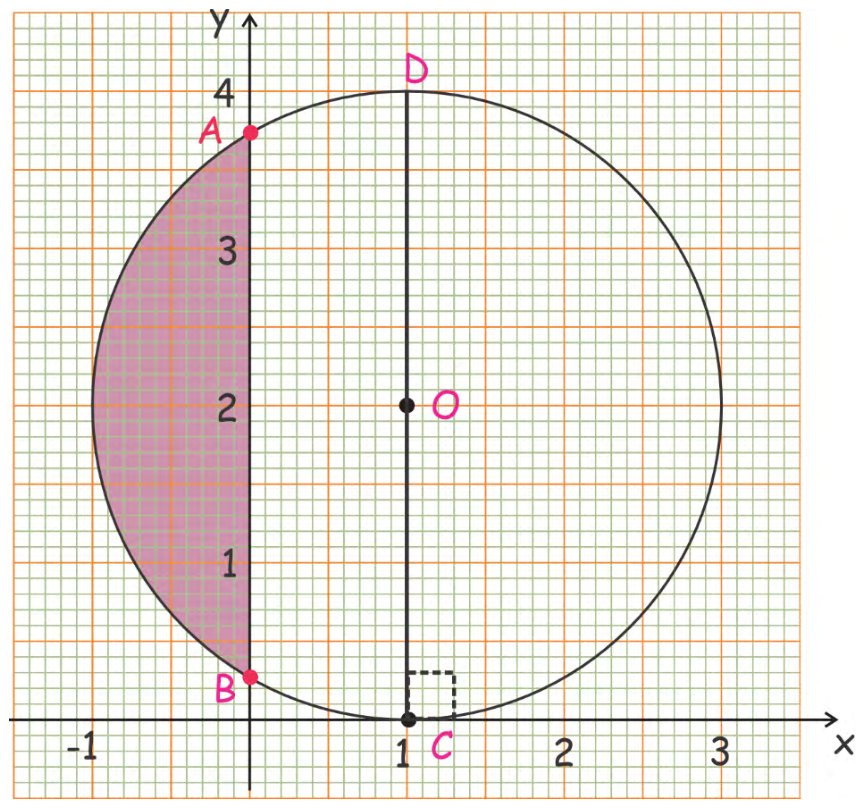
\includegraphics[width=0.6\linewidth]{figures/fig4-2.jpg}
\end{center}
\figcaption{4.2}{A circle}

The diameter is an example of a chord. It is the longest chord. The diameter is a
straight line from a point on the circumference through the centre to another point
on the circumference of the circle. In the above diagram, line COD is a diameter.

The $x$-axis is tangent to the circle at point C(1, 0). The tangent touches the circle
at one point. The angle between the tangent and the radius or the diameter at the
point of tangency is $90^\circ$. In the diagram OCX $= 90^\circ$

The area, shaded red, between the arc AB and the line AB is called a segment.

\begin{center}
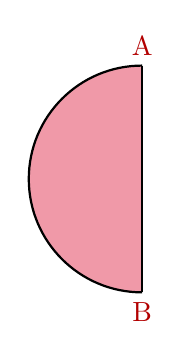
\begin{tikzpicture}[scale=0.9]
  \fill[red!40!purple!40] (0,-1.6) arc (270:90:1.6) -- cycle;
  \draw[black, thick] (0,-1.6) arc (270:90:1.6);
  \draw[black, thick] (0,1.6) -- (0,-1.6);
  \node[red!70!black, above] at (0,1.6) {A};
  \node[red!70!black, below] at (0,-1.6) {B};
\end{tikzpicture}
\end{center}
\figcaption{4.3}{A segment}

The area bounded by the arc AB and the lines OA and OB is called a sector.

\begin{center}
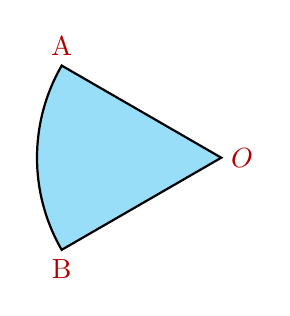
\begin{tikzpicture}[scale=0.9]
  \coordinate (O) at (0,0);
  \fill[cyan!40] (O) -- (150:2.6) arc (150:210:2.6) -- cycle;
  \draw[black, thick] (O) -- (150:2.6) arc (150:210:2.6) -- cycle;
  \node[red!70!black, right] at (O) {$O$};
  \node[red!70!black, above] at (150:2.6) {A};
  \node[red!70!black, below] at (210:2.6) {B};
\end{tikzpicture}
\end{center}
\figcaption{4.4}{A sector}

\begin{example}{Example 4.1}
The diagram below shows the graph of a circle. Use it to answer the questions.
\begin{center}
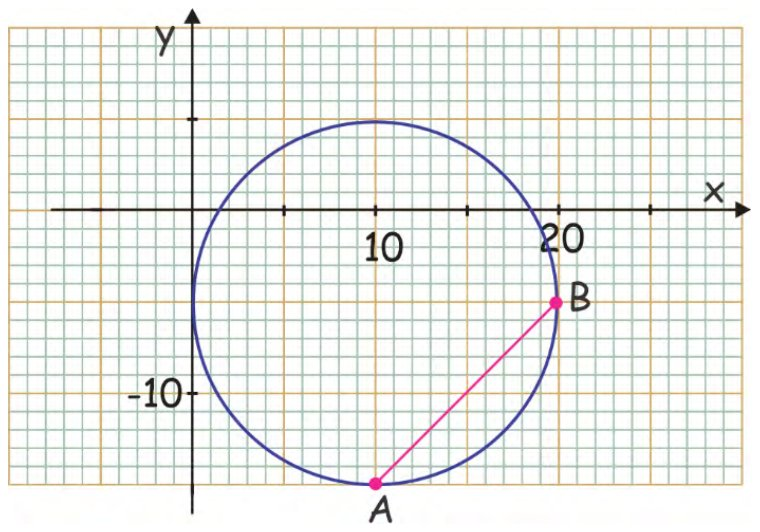
\includegraphics[width=0.55\linewidth]{figures/fig4-5.jpg}
\end{center}
\figcaption{4.5}{Graph of a circle}
\begin{enumerate}
  \item[a.] State the coordinates of the centre.
  \item[b.] Find the radius of the circle
  \item[c.] Find the length of chord AB
\end{enumerate}

\solution
\begin{enumerate}
  \item[a.] Coordinate of the centre is (10, -5)
  \item[b.] The radius of the circle is 10 units
  \item[c.] The coordinate of point A is (10, -15) and that of B is (20, -5)
  \item[d.] $|AB| = \sqrt{(20 - 10)^2 + (-5 \text{---} 15)^2}$
  \item[e.] $|AB| = \sqrt{10^2 + 10^2}$
  \item[f.] $= \sqrt{100 + 100}$
  \item[g.] $= \sqrt{200}$
  \item[h.] $= \sqrt{100 \times 2}$
  \item[i.] $= \sqrt{100} \times \sqrt{2}$
  \item[j.] $= 10\sqrt{2}$ units.
\end{enumerate}
\booknote[S4-01]{the working of part (c) is lettered d.\ to j.\ in the book as if
it were seven further parts; the question has only parts a--c.}
\booknote[S4-02]{the second bracket is printed ``$(-5\text{---}15)^2$''; it should
read $(-5 - (-15))^2 = 10^2$, as the next line shows.}
\end{example}
